\documentclass[
	% -- opções da classe memoir --
	12pt,				% tamanho da fonte
	openright,			% capítulos começam em pág ímpar (insere página vazia caso preciso)
	oneside,			% para impressão em frente e verso. Oposto a oneside
	a4paper,			% tamanho do papel.
	% -- opções da classe abntex2 --
	chapter=TITLE,		% títulos de capítulos convertidos em letras maiúsculas
	%section=TITLE,		% títulos de seções convertidos em letras maiúsculas
	%subsection=TITLE,	% títulos de subseções convertidos em letras maiúsculas
	%subsubsection=TITLE,% títulos de subsubseções convertidos em letras maiúsculas
	% -- opções do pacote babel --
	english,			% idioma adicional para hifenização
	french,				% idioma adicional para hifenização
	spanish,			% idioma adicional para hifenização
	brazil				% o último idioma é o principal do documento
	]{abntex2}
% ---
% Pacotes básicos 
% ---
\usepackage{lmodern}			% Usa a fonte Latin Modern
\usepackage{mathptmx}			% Usa a fonte Times New Roman
\usepackage[T1]{fontenc}		% Selecao de codigos de fonte.
\usepackage[utf8]{inputenc}		% Codificacao do documento (conversão automática dos acentos)
\usepackage{lastpage}			% Usado pela Ficha catalográfica
\usepackage{indentfirst}		% Indenta o primeiro parágrafo de cada seção.
\usepackage{color}				% Controle das cores
\usepackage{graphicx}			% Inclusão de gráficos
\usepackage{subcaption}				% Inclusão de gráficos lado a lado
\usepackage{microtype} 			% para melhorias de justificação
\usepackage{tabularx,ragged2e}	% Para inserir tabelas
\usepackage{multirow}			% Para mesclar células
\usepackage[dvipsnames,table,xcdraw]{xcolor}		% Permite adicionar cores nas linhas de tabelas
\usepackage{fancyvrb}			% Permite adicionar arquivos de texto
\usepackage[portuguese, ruled, linesnumbered]{algorithm2e} % Uso de algoritmos
\usepackage{amsfonts}			% Permite usar notação de conjuntos
\usepackage{amsmath}			% Permite citar equações
\usepackage{amsthm}				% Permite criar teoremas e experimentos
\usepackage[font={bf, small}, labelsep=endash, labelfont=bf]{caption}	% Faz legenda de figuras ficarem em negrito
\usepackage{cancel}				% Permite fazer expressão tendendo a zero
\usepackage{epstopdf}			% Converte eps para pdf
\usepackage[final]{pdfpages}
\usepackage{hyperref}
\usepackage{fancybox}


\newcolumntype{L}{>{\RaggedRight\arraybackslash}X}
% ---
% ---
% Pacotes adicionais, usados apenas no âmbito do Modelo Canônico do abnteX2
% ---
\usepackage{lipsum}				% para geração de dummy text
% ---
% ---
% Pacotes de citações
% ---
%\usepackage[brazilian,hyperpageref]{backref}	 % Paginas com as citações na bibl
\usepackage[alf, abnt-emphasize=bf]{abntex2cite}	% Citações padrão ABNT
% ---
% Customizações para o layout da UFPA
% ---
\usepackage{modelo-ufpa/ufpa}
% Muda o título de lista de ilustrações para lista de figuras
\addto\captionsbrazil{%
  \renewcommand{\listfigurename}%
    {Lista de Ilustrações}%
	\renewcommand{\listtablename}%
    {Lista de Tabelas}%
}
% Permite utilizar figuras sem precisar colocar o caminho absoluto
\graphicspath{{imagens/}}
% Define o ambiente de experimentos
\theoremstyle{definition}
\newtheorem{experimento}{Experimento}[section]
\newcommand{\experimentoautorefname}{Experimento}


% --------------------------------------------------------------
% Informações do TRABALHO
% --------------------------------------------------------------
\universidade{UNIVERSIDADE FEDERAL DO PARÁ}
\instituto{INSTITUTO DE TECNOLOGIA}
\faculdade{FACULDADE DE COMPUTAÇÃO E TELECOMUNICAÇÕES}
%\curso{CURSO DE BACHARELADO EM SISTEMAS DE INFORMAÇÃO}
\titulo{RELATÓRIO DE SISTEMAS OPERACIONAIS}
\autor{
%\begin{tabular}{l l}
    DAVID PINHEIRO DE SOUSA - 202207040045 \\
    JOAO VICTOR SANTOS BRITO FERREIRA - 202207040028 \\
    JOEL TAVARES MIRANDA - 202206840054 \\
    KAUAN MIRANDA TAVARES - 202206840033 \\
    MARCO ANTONIO DO ESPIRITO SANTO MAUES JUNIOR - 202206840038 \\
%\end{tabular}
}
\local{Belém}
\data{2023}
\orientador{Prof. Dr. Diego Lisboa Cardoso}
\tipotrabalho{Monografia}

% o nome da instituição e a área de concentração 
\preambulo{Relatório do trabalho 1 de Sistemas Operacionais.}
%\sobrenome{Sobrenome}
%\nome{Nome}
%\palavraschave
%\datadadefesa{Data da Defesa: 09 de Março de 2017}%07 de Dezembro de 2016}
\conceito{Conceito: Excelente}
\faculdadedoorientador{Faculdade de  - UFPA}
\primeiromembrodabanca{Prof. Dr. Nome Sobrenome}
\faculdadedoprimeiromembrodabanca{Faculdade de  - UFPA}
\segundomembrodabanca{Prof. Dra. Nome Sobrenome}
\faculdadedosegundomembrodabanca{Faculdade de  - UFPA}
% -------------------------------------------------------------------------
% ---
% Configurações de aparência do PDF final
% alterando o aspecto da cor azul
\definecolor{blue}{RGB}{41,5,195}
% informações do PDF
\makeatletter
\hypersetup{
     	%pagebackref=true,
		pdftitle={\imprimirtitulo}, 
		pdfauthor={\imprimirautor},
    	pdfsubject={\imprimirpreambulo},
	    pdfcreator={LaTeX with abnTeX2},
		pdfkeywords={\imprimirpalavraschave}, 
		colorlinks=true,       		% false: boxed links; true: colored links
    	linkcolor=black,          	% color of internal links
    	citecolor=black,        		% color of links to bibliography
    	filecolor=magenta,      		% color of file links
		urlcolor=blue,
		bookmarksdepth=4,
        breaklinks=true
}
\makeatother
% --- 
% Espaçamentos entre linhas e parágrafos 
% --- 
% O tamanho do parágrafo é dado por:
\setlength{\parindent}{1.3cm}
% Controle do espaçamento entre um parágrafo e outro:
\setlength{\parskip}{0.2cm}  % tente também \onelineskip
% compila o indice
% ---
\makeindex
% ---

% -------------------------------------------------------------------------
% ---------------------------INICIO DO DOCUMENTO---------------------------
% -------------------------------------------------------------------------
\begin{document}
% Seleciona o idioma do documento (conforme pacotes do babel)
\selectlanguage{brazil}
% Retira espaço extra obsoleto entre as frases.
\frenchspacing 
% ----------------------------------------------------------
% ELEMENTOS PRÉ-TEXTUAIS
% ----------------------------------------------------------
% \pretextual

% ---
% Capa
% ---
\imprimircapa
% ---

% ---
% Folha de rosto

\imprimirfolhaderosto

\newpage

\setlength{\absparsep}{18pt} % ajusta o espaçamento dos parágrafos do resumo

\pdfbookmark[0]{\contentsname}{toc}
\tableofcontents*
\cleardoublepage
% ---
% ---------------------------------------------------------
% ELEMENTOS TEXTUAIS
% ----------------------------------------------------------
\textual

% ----------------------------------------------------------
% Introdução
% ----------------------------------------------------------

\chapter{Introdução}

A computação de baixo nível desempenha um papel fundamental na compreensão 
do funcionamento interno dos sistemas de computação. Para aprofundar nosso entendimento 
desse aspecto, este relatório descreve o desenvolvimento e a execução de um programa 
em Assembly x86, cujo propósito é demonstrar a manipulação básica de dados,
operações aritméticas e a interação com o sistema operacional por meio de chamadas de sistema.
\chapter{Objetivos}

O objetivo deste projeto é criar um programa em C e Assembly x86 que:

\begin{itemize}
	\item \textbf{Solicita Entradas do Usuário}:
	  \begin{itemize}
		\item A chamada de sistema \ovalbox{sys\_read} será utilizada para ler os números fornecidos pelo usuário a partir 
		da entrada padrão (\ovalbox{stdin}).
	  \end{itemize}
	\item \textbf{Realiza Operações Aritméticas}:
	  \begin{itemize}
		\item As operações aritméticas de soma e subtração serão realizadas diretamente no código Assembly 
		x86, sem a necessidade de chamadas de sistema específicas para essas operações.
	  \end{itemize}
	\item \textbf{Exibe Resultados}:
	  \begin{itemize}
		\item A chamada de sistema \ovalbox{sys\_write} será usada para exibir os resultados das operações de 
		soma e subtração na saída padrão (\ovalbox{stdout}).
	  \end{itemize}
	\item \textbf{Encerra de Forma Adequada}:
	  \begin{itemize}
		\item O programa encerrará de maneira apropriada usando a chamada de sistema \ovalbox{sys\_exit} para 
		indicar o término bem-sucedido da execução com um código de saída igual a 0.
	  \end{itemize}
  \end{itemize}
  

\chapter{Desenvolvimento (Programa explicado e Cópias das telas do emulador.)}

Primeiramente, o desenvolvimento deste projeto envolveu a criação de um programa em C, 
posteriormente convertido para Assembly x86\_64,  que
permitisse a realização de operações de soma e subtração, com a possibilidade de interação 
com o usuário. A principal funcionalidade do programa é determinar se o usuário deseja somar
ou subtrair dois números, calcular o resultado e exibi-lo na tela através das chamadas de sistema propostas. 
O ambiente de desenvolvimento escolhido para esta implementação foi o Visual Studio Code, uma ferramenta popular para 
desenvolvimento de código e a execução do programa ocorreu no ambiente do Ubuntu, utilizando o
terminal Zsh. Isso proporcionou um ambiente familiar e prático para a execução e teste do programa, 
bem como a captura de informações para este relatório.

\section{Implementação em C}

A implementação em C foi desenvolvida para fornecer uma funcionalidade simples de soma e subtração com 
interação do usuário. Abaixo, detalhamos a implementação em C, com foco no uso de chamadas de sistema 
para interagir com o sistema operacional.

\subsection{Código}

O código-fonte em C utiliza bibliotecas padrão, como \ovalbox{stdio.h} e \ovalbox{unistd.h}, 
para realizar operações de entrada e saída. A seguir, apresentamos uma visão geral do código em C:

\begin{verbatim}
#include <stdio.h>
#include <unistd.h> // Para as chamadas de sistema read e write
#include <stdlib.h> // Para a chamada exit

int main() {
    // ... (definição de variáveis e inicialização)

    // Mensagem de prompt
    char prompt[] = "Digite 1 para soma e 2 para subtração\n";
    write(STDOUT_FILENO, prompt, sizeof(prompt) - 1); // Chamada de sistema para 
	// escrever na tela

    // Leitura da entrada
    char input_buffer[10]; // Buffer para a entrada
    int bytes_read = read(STDIN_FILENO, input_buffer, sizeof(input_buffer));
    // ... (lógica de entrada e validação)

    // Lógica para soma ou subtração
    if (soma_ou_sub == 1) {
        // ... (lógica de soma)
    } 
    else {
        // ... (lógica de subtração)
    }
    // ... (exibição de resultados)

    exit(0);
    return 0;
}
\end{verbatim}

\subsection{Uso de Chamadas de Sistema}

O código em C faz uso explícito de chamadas de sistema para realizar operações de entrada e saída. 
Aqui estão alguns exemplos destacados:

\begin{itemize}
    \item \textbf{write(STDOUT\_FILENO, prompt, sizeof(prompt) - 1)}: Essa chamada de sistema 
	escreve a mensagem de prompt na saída padrão (normalmente a tela). O descritor de arquivo 
	\ovalbox{STDOUT\_FILENO} é usado para referenciar a saída padrão.

    \item \textbf{read(STDIN\_FILENO, input\_buffer, sizeof(input\_buffer))}: Essa chamada de 
	sistema lê a entrada do usuário da entrada padrão (normalmente o teclado) para o \ovalbox{input\_buffer}.

    \item \textbf{exit(0)}: Esta chamada de sistema encerra o programa e retorna um código de 
	saída de 0 para indicar que a execução foi bem-sucedida.

\end{itemize}

A implementação em C demonstra claramente o uso das chamadas de sistema para interagir com o 
sistema operacional, permitindo a comunicação com o usuário e a manipulação de dados de entrada e saída.

\subsection{Execução}

Para executar o código em C foi utilizado o comando 
\ovalbox{gcc soma\_e\_subtração.c -o soma\_e\_subtração}
e então é criado um executável do programa que é executado
através do comando \ovalbox{./soma\_e\_subtração}.

Na figura~\ref{fig:run_c}, é mostrada a execução do programa em C no ambiente Ubuntu com o Zsh no terminal do Visual Studio 
Code, destacando o uso das chamadas de sistema para interação com o sistema operacional e validando a implementação em C.

\begin{figure}
    \centering
    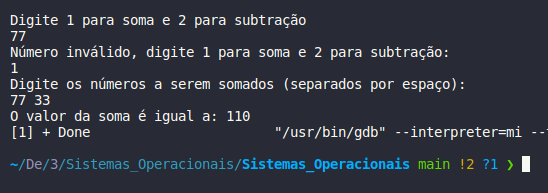
\includegraphics[width=1.0\textwidth]{imagens/run_c.png}
	\caption{Execução no terminal do código em C.}
	\label{fig:run_c}
\end{figure}

\section{Implementação em Assembly x86\_64}

A implementação em Assembly x86\_64 foi gerada a partir do código-fonte em C usando o comando 
\ovalbox{gcc -S}. O código Assembly resultante foi cuidadosamente adaptado para garantir que ele 
mantenha a mesma funcionalidade que o programa em C. Abaixo, apresento uma descrição detalhada da 
implementação em Assembly, com ênfase no uso das chamadas de sistema para interagir com o sistema operacional.

\subsection{Diretivas e Seções}

O código Assembly começa com diretivas e seções que definem informações essenciais do programa, 
como seções de texto e dados, bem como informações de depuração.

\begin{verbatim}
    .section .rodata
.LC0:
    .string "%d"
.LC1:
    .string "%d %d"
    ...
\end{verbatim}

\subsection{Inicialização e Manipulação de Dados}

A implementação em Assembly inicia com a inicialização de variáveis e buffers para 
armazenar dados de entrada e saída. Isso inclui a configuração de buffers para entrada de 
usuário e para a exibição de resultados.

\begin{verbatim}
    .data
    .align 8
prompt_input:
    .string "Digite 1 para soma e 2 para subtração\n"
...
\end{verbatim}

\subsection{Interação com o Usuário}

Assim como no código em C, o programa em Assembly interage com o usuário, exibindo 
mensagens de prompt e lendo a entrada do usuário. Ele utiliza chamadas de sistema 
para realizar essas operações.

\begin{verbatim}
    leaq    prompt_input(%rip), %rdi
    call    printf
    leaq    input_buffer(%rip), %rdi
    leaq    input_format(%rip), %rsi
    call    __isoc99_sscanf@PLT
\end{verbatim}

\subsection{Lógica de Soma e Subtração}

A implementação em Assembly inclui a lógica para realizar as operações de soma e 
subtração com os números fornecidos pelo usuário. Os resultados são calculados e 
armazenados em variáveis temporárias.

\begin{verbatim}
    movl    -220(%rbp), %edx
    movl    -216(%rbp), %eax
    addl    %edx, %eax
    movl    %eax, -208(%rbp)
\end{verbatim}

\subsection{Formatação e Exibição}

Após calcular o resultado, o programa em Assembly formata as mensagens de saída de acordo 
com o resultado da operação (soma ou subtração). As mensagens formatadas são exibidas na 
tela usando chamadas de sistema.

\begin{verbatim}
    leaq    result_output(%rip), %rdi
    call    printf
\end{verbatim}

\subsection{Manipulação de Erros}

O código Assembly inclui tratamento de erros para casos em que a entrada do usuário não é 
válida. Isso é feito usando desvios condicionais e mensagens de erro apropriadas.

\begin{verbatim}
    cmpl    $2, -220(%rbp)
    jne     .L7
\end{verbatim}

\subsection{Execução}

\begin{figure} %corrigir aqui
    \centering
    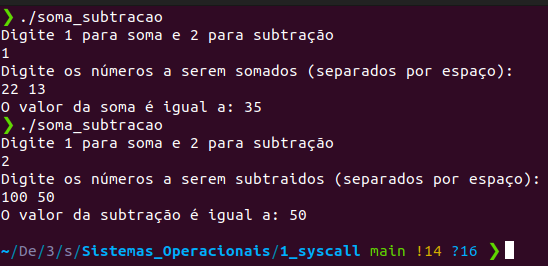
\includegraphics[width=1.0\textwidth]{imagens/run_asm.png}
	\caption{Execução no terminal do código em Assembly!!!!!!!!!!!!!!!!!!!!!!!!.}
	\label{fig:run_asm}
\end{figure}

%A implementação em Assembly foi desenvolvida com ênfase no uso das chamadas de sistema 
%para interagir com o sistema operacional, permitindo que o programa seja executado em um 
%ambiente de sistema operacional, como o Ubuntu, como mencionado anteriormente.

Para executar o código em assembly foi utilizado o seguinte comando no terminal 
\ovalbox{gcc -o soma\_e\_subtração soma\_e\_subtração.s}
e então é criado um executável do programa que é executado através do comando \ovalbox{./soma\_e\_subtração}.
 
Na figura~\ref{fig:run_asm}, é mostrada a execução do programa em 
Assembly no ambiente Ubuntu com o Zsh, destacando o uso das chamadas de sistema para 
interação com o sistema operacional e validando a implementação em Assembly.

\section{Capturas da IDE mostrando o código}

Nesta seção serão apresentadas capturas da tela da IDE mostrando os códigos em C e 
Assembly que já foram apresentados e explicados ao longo do trabalho. Os códigos 
apresentados estão disponíveis tambem em 
\href{https://github.com/jvictorferreira3301/Sistemas_Operacionais}{nosso repositório da disciplina}


\begin{figure}
	\centering
	\begin{minipage}{1.0\textwidth}
	  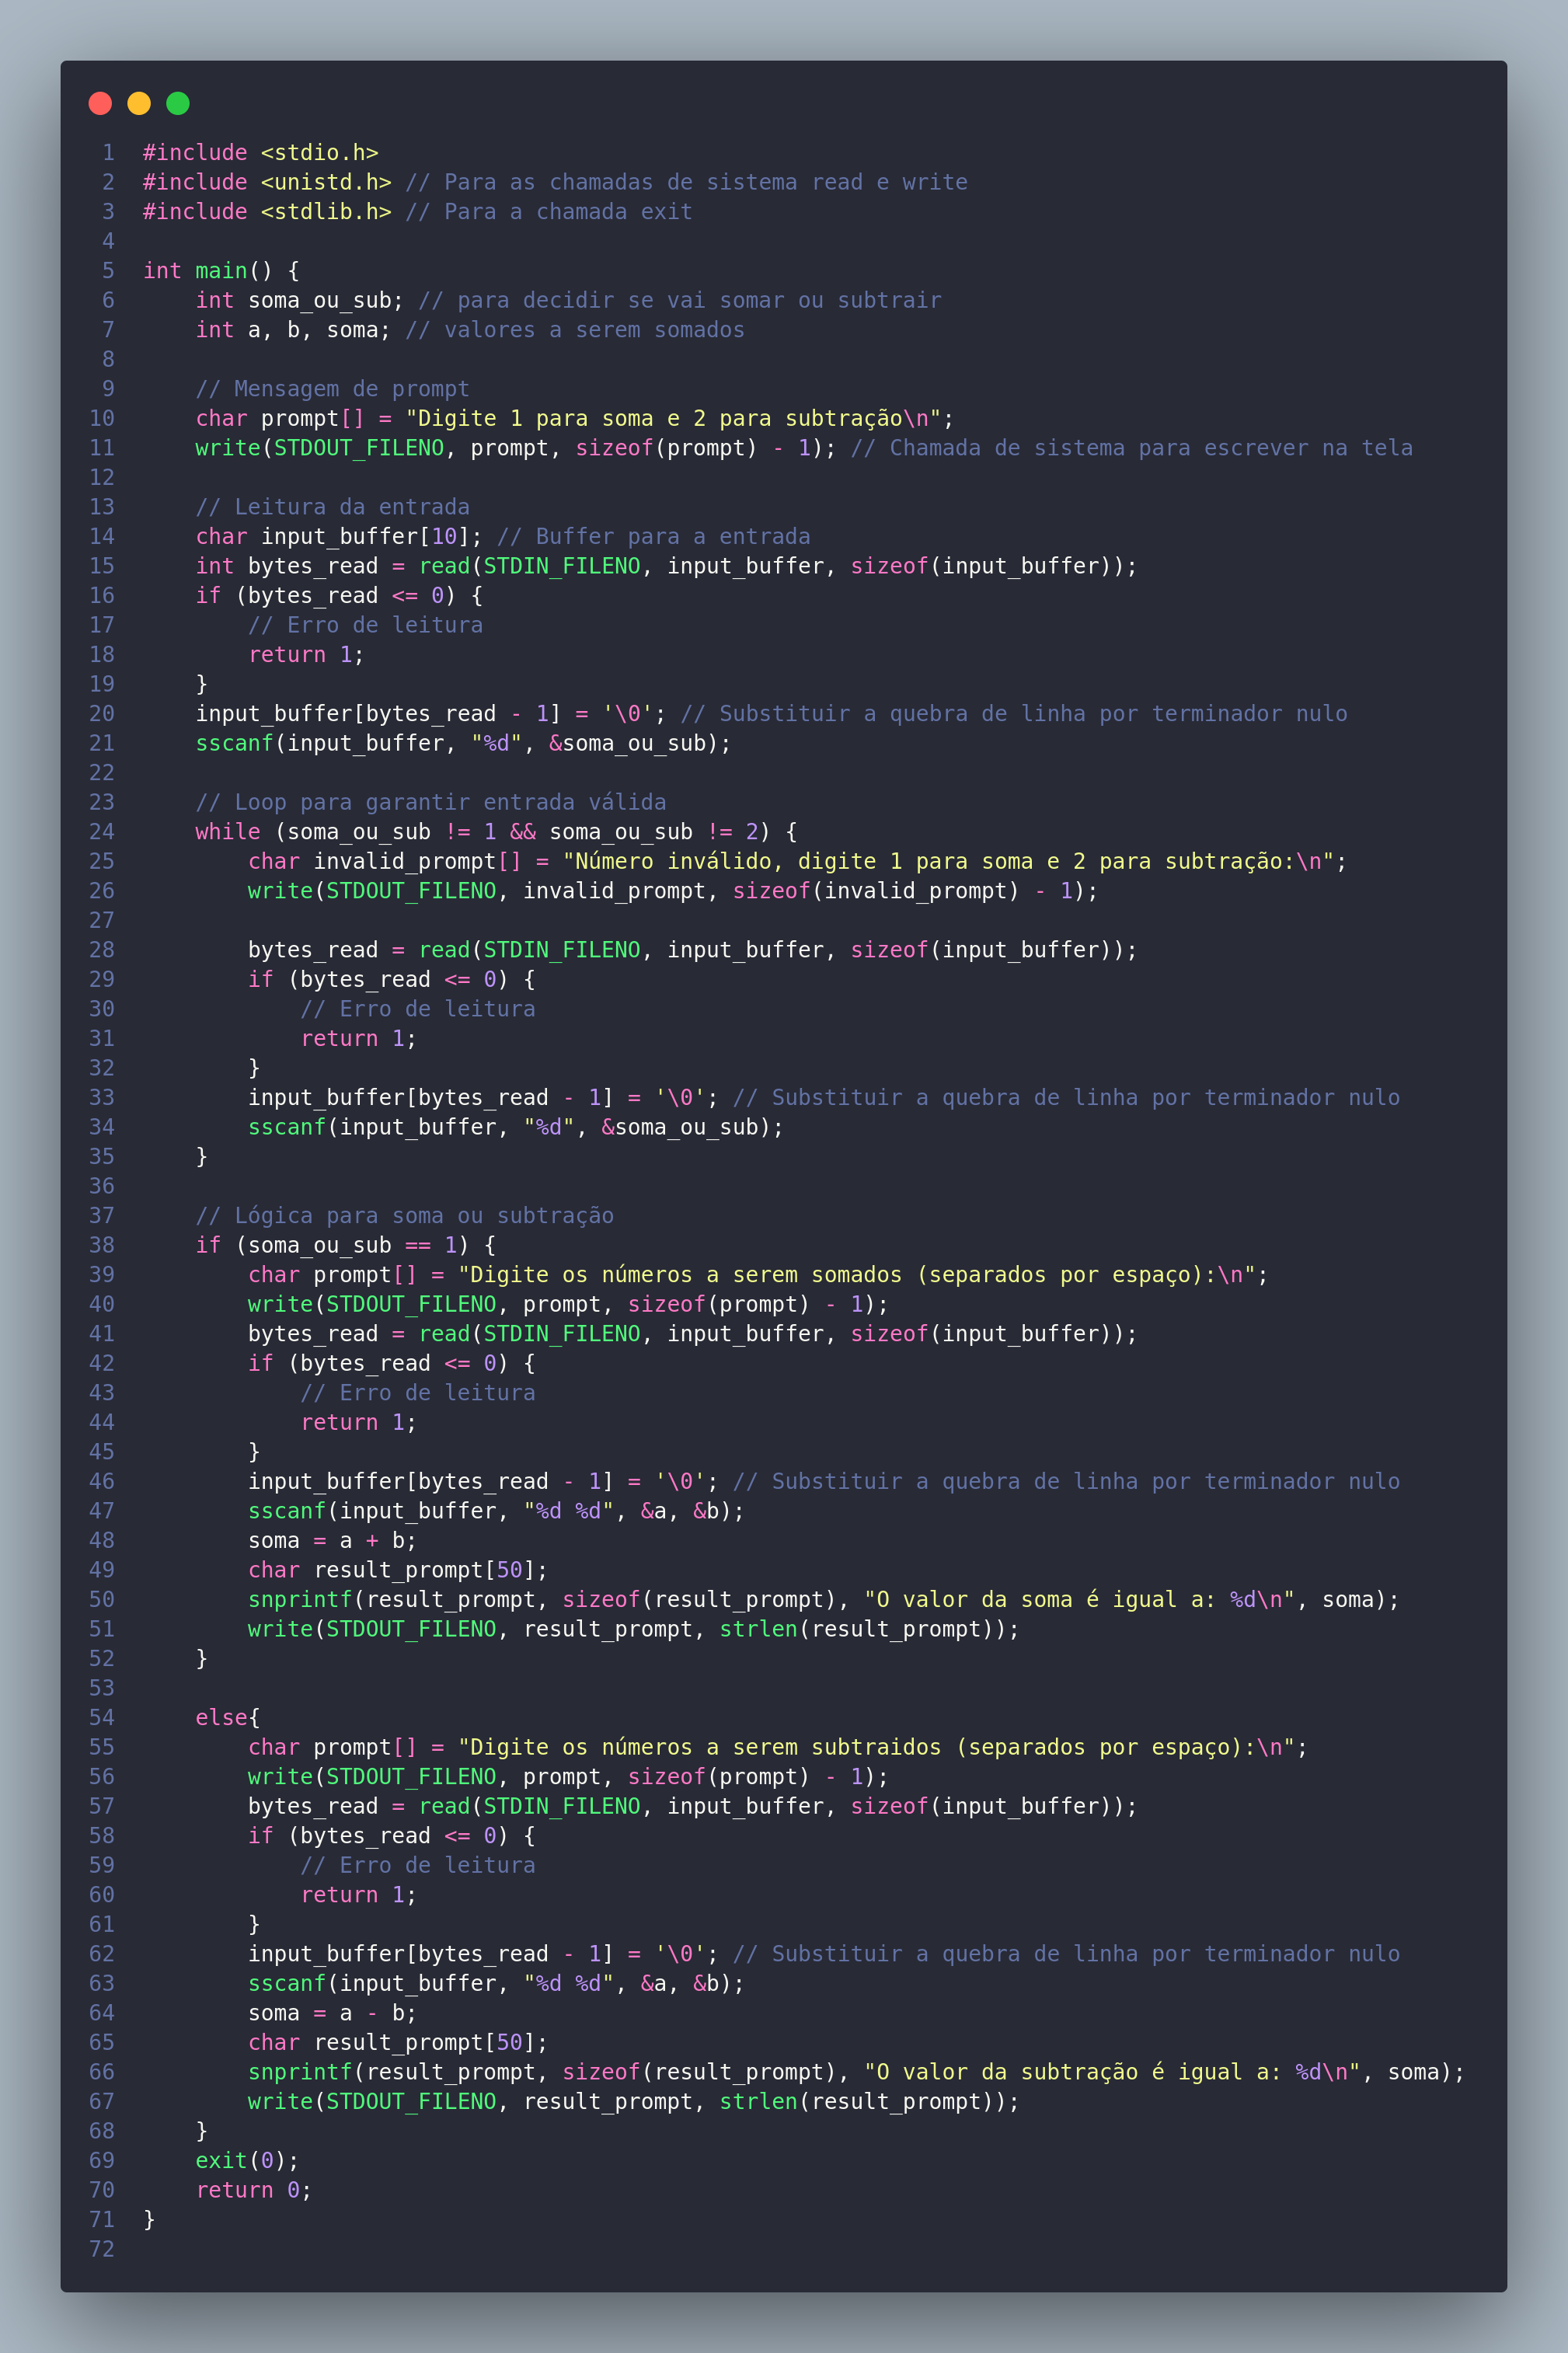
\includegraphics[width=1.0\linewidth]{imagens/code_c.png}
	  \caption{Código em C. Disponível em: \href{https://github.com/jvictorferreira3301/Sistemas_Operacionais}{github.com/jvictorferreira3301/SistemasOperacionais}}
	\end{minipage}
\end{figure}

Por conta do código em Assembly ser muito extenso optamos por apresentar o mesmo em \href{https://github.com/jvictorferreira3301/Sistemas_Operacionais/blob/main/1_syscall/soma_subtracao.s}
{github.com/jvictorferreira3301/Sistemas\_Operacionais/blob/main/1\_syscall/soma\_subtracao.s}

\chapter{Conclusão}
\label{conclusao}


Este projeto permitiu uma exploração prática de conceitos fundamentais relacionados 
à programação em Assembly x86, operações 
aritméticas, manipulação de dados e interação com o sistema operacional por meio de 
chamadas de sistema que é um conceito ministrado na disciplina em questão. 
Ao criar um programa simples que solicita
entradas do usuário, realiza operações de soma e subtração e exibe os resultados, 
pudemos destacar a importância das chamadas de sistema no 
desenvolvimento de aplicativos de baixo nível e por em prática o exposto nas aulas.

Ao longo do projeto, observamos como as chamadas de sistema 
\ovalbox{sys\_read},\ovalbox{sys\_write} e \ovalbox{sys\_exit}
desempenham papéis cruciais na execução de tarefas essenciais.
 
A \ovalbox{sys\_read} permitiu a entrada de dados pelo usuário, enquanto a \ovalbox{sys\_write} 
facilitou a saída dos resultados na tela. A \ovalbox{sys\_exit} garantiu um encerramento 
adequado do programa, indicando que a execução foi bem-sucedida.

Além disso, este projeto serviu como uma introdução valiosa à programação Assembly x86, uma 
linguagem de baixo nível que é essencial para compreender o funcionamento interno dos sistemas de 
computação. A manipulação direta de registradores e a realização de operações aritméticas sem a 
abstração das linguagens de alto nível nos deram uma apreciação mais profunda do 
funcionamento interno do hardware.


\postextual

\bibliography{bibliografia}

\cite{tanenbaum2010sistemas}

\end{document}
